\section{Implementarea plugin-ului audio} 
    \label{plugin}
    \noindent Plugin-ul audio este implementat în C++ folosind framework-ul JUCE, împreună cu modulul PluginGuiMagic  \cite{website:1}. Clasa MagicProcessor din modulul PluginGuiMagic extinde clasa AudioProcessor și reprezintă clasa de bază din care este derivat punctul de început al plugin-ului.
    \begin{figure}[H]
        \centering
        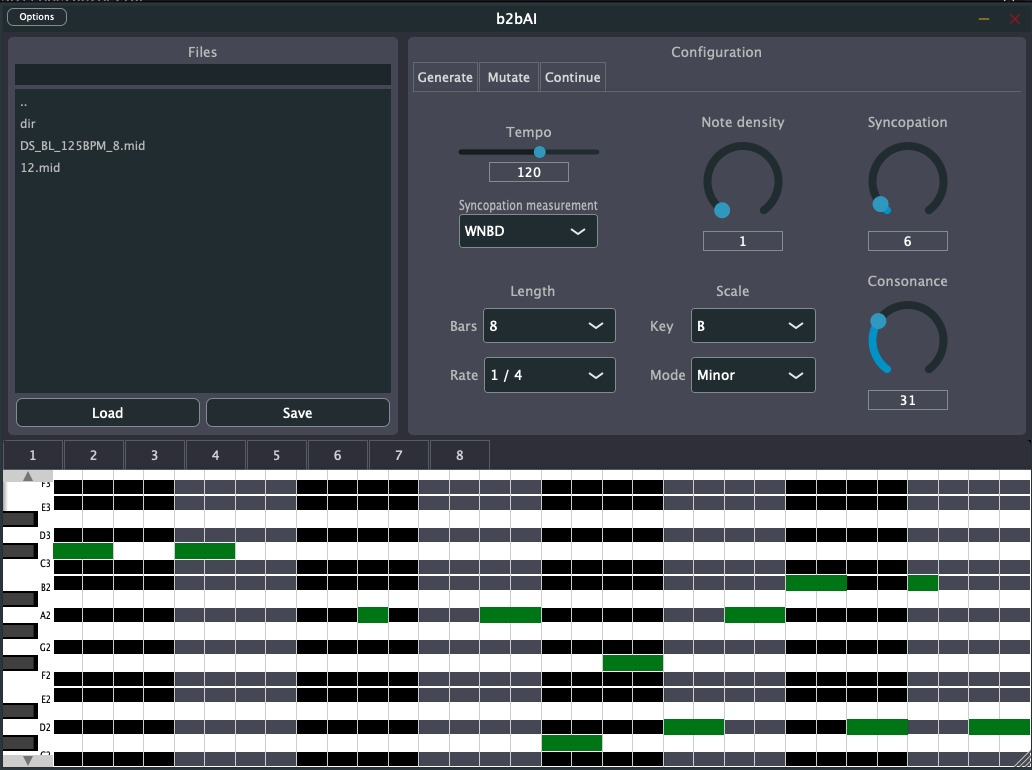
\includegraphics[scale=0.3]{images/interfata.jpeg}
        \caption{Interfața grafică a plugin-ului}
        \label{fig:interfata}
    \end{figure}
    \subsection{B2bAIPluginProcessor}
    \noindent Interfața grafică a plugin-ului este creată dintr-un fișier XML, care conține o structură arborescentă de componente (Anexa \ref{XML}). Acesta este încarcat în constructor-ul clasei B2bAIPluginProcessor (Anexa \ref{B2bAIAudioProcessor}), care extinde clasa MagicProcessor și reprezintă componenta principală a plugin-ului. Clasa crează de asemenea parametrii audio și celelalte resurse dinamice și le atașează componentelor corespunzătoare. În plus, aceasta recepționează și procesează mesaje MIDI și evenimente audio. \par
    Metoda initialiseBuilder, care suprascrie metoda virtuală a clasei MagicProcessor, permite înregistrarea de componente noi refolosibile.
    \begin{minted}[fontsize=\footnotesize, baselinestretch=1]{c++}
void B2bAIAudioProcessor::initialiseBuilder 
                            (foleys::MagicGUIBuilder& builder)
{
    builder.registerJUCEFactories();

    builder.registerFactory ("PianoRoll", &PianoRoll::factory);
    builder.registerFactory ("SearchBar", &SearchBar::factory);
}
    
    \end{minted}
    \subsection{Piano roll}
        \noindent Piano roll-ul permite vizualizarea și editarea notelor dintr-o secvență. Opt secvențe pot fi editate simultan; pentru a încarcă o secventă în piano roll se folosesc tab-urile numerotate de la 1 la 8. Notele pot fi adaugate, șterse,  mutate sau redimensionate pe grid folosind mouse-ul, valorile notelor (tonice) pot fi derulate folosind mousewheel-ul. \par
        Piano roll-ul este implementat folosind clasa PianoRollComponent (Anexa \ref{PianoRollComponent}), care încapsulează 2 componente: un pian (KeyboardComponent) și un un grid (GridComponent). Pianul este un reskin al componentei JUCE::MidiKeyboardComponent. Grid-ul este o matrice construită dinamic în funcție de evenimentele generate de mouse, numărul de pulsuri al metrului și o listă de note inițializată la runtime (Anexa \ref{Update}). \par 
                \begin{figure}[H]
            \centering
            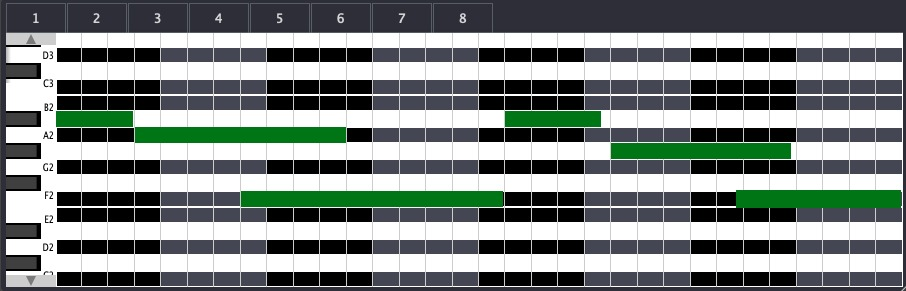
\includegraphics[scale=0.428]{images/pianoroll.jpeg}
            \caption{Piano roll}
            \label{fig:piano_rol}
        \end{figure}
        \noindent Wrapper-ul PianoRoll (Anexa \ref{PianoRoll}) încapsulează această clasă PianoRollComponent și este folosit pentru a o înregistra drept componentă reutilizabilă în B2bAIAudioProcessor::initialiseBuilder. În plus, wrapperul prezintă și o interfață pentru a inițializa și actualiza referința către lista de note din grid. \par
        
        \begin{figure}[H]
            \centering
            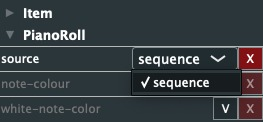
\includegraphics[scale=0.6]{images/interface.jpeg}
            \caption{Selectarea secvenței din piano roll}
            \label{fig:interface}
        \end{figure}
        
    \subsection{Sistemul de fișiere}
        \noindent Sistemul fișier de interne poate fi navigat din aplicației. Secvența MIDI asociată piano roll-ului poate fi salvată ca fișier intern. De asemenea un fișier în format MIDI poate fi descărcat și editat în piano roll.
        \begin{figure}[H]
            \centering
            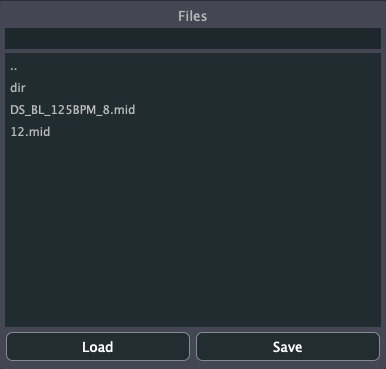
\includegraphics[scale=0.5]{images/files.jpeg}
            \caption{File tree}
            \label{fig:files}
        \end{figure}
        \noindent Implementarea este realizată folosind clasa MidiFileListBox (Anexa \ref{MidiFileListBox}), care extinde clasele ListBoxModel, ChangeBroadcaster, ChangeListener și Label::Listener. Astfel, aceasta definește 3 funcții care sunt implementate în procesorul audio, care modifică setările comune ale aplicației, și actualizează starea componentelor interioare de fiecare dată când sunt apelate. În plus, acest lucru se întâmplă și pentru chenarul de deasupra, actualizarea având loc în momentul în care este schimbată valoarea din chenar. Chenarul este definit în clasa SearchBar (Anexa \ref{SearchBar}) și este înregistrat drept componentă reutilizabilă.
    \subsection{Parametrii audio}
        \noindent Parametrii audio ai aplicației sunt folosiți pentru a configura algoritmul genetic. Fiecare dintre cele 4 funcționalități ale aplicației are parametrii de configurație proprii. \par
        \noindent \textbf{Generate}
        \begin{itemize}
            \item Syncopation - nivelul de sincopare
            \item Note density - densitatea notelor
            \item Consonance - proporția notelor consonante
            \item Key - gama în care este generată secvența
            \item Mode - modul gamei
            \item Tempo - tempo-ul secvenței; este folosit în scrierea fișierelor midi
            \item Bars - numărul de măsuri al secvenței
            \item Rate - durata unui puls
            \item Syncopation measurement - algoritmul folosit pentru măsurarea sincopării 
        \end{itemize}
        \noindent \textbf{Mutate}
        \begin{itemize}
            \item Pitch - rata de mutație a frecvenței
            \item Velocity - rata de mutație a velocității
            \item Duration - rata de mutație a lungimilor notelor
            \item Consonance - proporția notelor consonante
        \end{itemize}
        \noindent \textbf{Continue}
        \begin{itemize}
            \item Compression method: algoritmul folosit pentru compresia secvențelor
        \end{itemize}
        \noindent \textbf{Combine}
        \begin{itemize}
            \item Compression method: algoritmul folosit pentru compresia secvențelor
            \item Sequences: secvențele folosite în combinare
        \end{itemize}